\documentclass[10pt]{book}

%These tell TeX which packages to use.
\usepackage{array,epsfig}
\usepackage{amsmath}
\usepackage{amsfonts}
\usepackage{amssymb}
\usepackage{amsxtra}
\usepackage{amsthm}
\usepackage{mathrsfs}
\usepackage{color}
\usepackage{enumitem}
%\usepackage{mdframed}
\usepackage[most]{tcolorbox}
\usepackage{pgfplots}
\usetikzlibrary{arrows}
\pgfplotsset{compat=1.6}

\pgfplotsset{soldot/.style={color=black,only marks,mark=*}} \pgfplotsset{holdot/.style={color=black,fill=white,only marks,mark=*}}

%Here I define some theorem styles and shortcut commands for symbols I use often
\theoremstyle{definition}
\newtheorem{defn}{Definition}
\newtheorem{thm}{Theorem}
\newtheorem{cor}{Corollary}
\newtheorem*{rmk}{Remark}
\newtheorem{lem}{Lemma}
\newtheorem*{joke}{Joke}
\newtheorem{ex}{Example}
\newtheorem*{soln}{Solution}
\newtheorem{prop}{Proposition}

\newcommand{\lra}{\longrightarrow}
\newcommand{\ra}{\rightarrow}
\newcommand{\surj}{\twoheadrightarrow}
\newcommand{\graph}{\mathrm{graph}}
\newcommand{\bb}[1]{\mathbb{#1}}
\newcommand{\Z}{\bb{Z}}
\newcommand{\Q}{\bb{Q}}
\newcommand{\R}{\bb{R}}
\newcommand{\C}{\bb{C}}
\newcommand{\N}{\bb{N}}
\newcommand{\M}{\mathbf{M}}
\newcommand{\m}{\mathbf{m}}
\newcommand{\MM}{\mathscr{M}}
\newcommand{\HH}{\mathscr{H}}
\newcommand{\Om}{\Omega}
\newcommand{\Ho}{\in\HH(\Om)}
\newcommand{\bd}{\partial}
\newcommand{\del}{\partial}
\newcommand{\bardel}{\overline\partial}
\newcommand{\textdf}[1]{\textbf{\textsf{#1}}\index{#1}}
\newcommand{\img}{\mathrm{img}}
\newcommand{\ip}[2]{\left\langle{#1},{#2}\right\rangle}
\newcommand{\inter}[1]{\mathrm{int}{#1}}
\newcommand{\exter}[1]{\mathrm{ext}{#1}}
\newcommand{\cl}[1]{\mathrm{cl}{#1}}
\newcommand{\ds}{\displaystyle}
\newcommand{\vol}{\mathrm{vol}}
\newcommand{\cnt}{\mathrm{ct}}
\newcommand{\osc}{\mathrm{osc}}
\newcommand{\LL}{\mathbf{L}}
\newcommand{\UU}{\mathbf{U}}
\newcommand{\support}{\mathrm{support}}
\newcommand{\AND}{\;\wedge\;}
\newcommand{\OR}{\;\vee\;}
\newcommand{\Oset}{\varnothing}
\newcommand{\st}{\ni}
\newcommand{\wh}{\widehat}
%Pagination stuff.
\setlength{\topmargin}{-0.75in}
\setlength{\oddsidemargin}{0in}
\setlength{\evensidemargin}{0in}
\setlength{\textheight}{9.in}
\setlength{\textwidth}{6.5in}
\pagestyle{empty}
\begin{document}
\begin{flushleft}
Name:\underline{\hspace{13cm}}Date:\underline{\hspace{2cm}}
\end{flushleft}
\begin{center}
{\Large Math 1041-012 \hspace{0.5cm} Section 4.1}
\end{center}
%\vspace{0.2 cm}

\begin{tcolorbox}
\subsection*{Definitions}
Let $c$ be a number in the domain $D$ of a function $f$. Then $f(c)$ is the
\begin{itemize}
    \item \textbf{absolute maximum} value of $f$ on $D$ if \underline{\hspace{3cm}} for all $x$ in $D$,
    \item \textbf{absolute minimum} value of $f$ on $D$ if \underline{\hspace{3cm}} for all $x$ in $D$.
\end{itemize}
The absolute max/min are also called global max/min or extreme values.\\ \\
\textit{Remark}: The absolute max/min maybe at the endpoints of an interval or inside an interval. A function may or may not have a max or min. You also need to consider the domain $D$ it could be closed, open, infinite, finite, this can affect whether we have abs. max/min.
\end{tcolorbox}
\subsection*{Example 1}
In each graph determine if there are absolute maxima or minima. Explain your response.\\ \\
\begin{tikzpicture}[scale=1]
\begin{axis}[
  axis x line=middle, axis y line=middle,xlabel={}, ylabel={},yticklabels={,,},xticklabels={,,},ytick=\empty,xtick=\empty,
  ymin=-1, ymax=1, 
  xmin=-1, xmax=1,
  axis line style={<->}, width=8cm
]
\addplot[<->,domain=-1:1,black]{x^3};
\end{axis}
\end{tikzpicture}\\ \\
\begin{tikzpicture}[scale=1]
\begin{axis}[
  axis x line=middle, axis y line=middle,xlabel={}, ylabel={},yticklabels={,,},xticklabels={,,},ytick=\empty,xtick=\empty,
  ymin=-0.25, ymax=1, 
  xmin=-1, xmax=1,
  axis line style={<->}, width=8cm
]
\addplot[<->,domain=-1:1,black]{x^2};
\end{axis}
\end{tikzpicture}
\begin{tcolorbox}
\subsection*{Definitions}
The number $f(c)$ is a
\begin{itemize}
    \item \textbf{local maximum} value of $f$ if \underline{\hspace{3cm}} when $x$ is near $c$,
    \item \textbf{local minimum} value of $f$ if \underline{\hspace{3cm}} when $x$ is near $c$.
\end{itemize}
\textit{Remark}: Local max/min points are never at endpoints! If abs. max/min are interior points, then they are also local max/min.\\ \\
Local max/min are not necessarily absolute max/min.
\end{tcolorbox}
\subsection*{Example 2} The graph of $f(x)$ is shown below. State the local maximum and minimum values of the function. For abs. max/min state whether it is an endpoint or interior point.
\begin{figure}[h]
    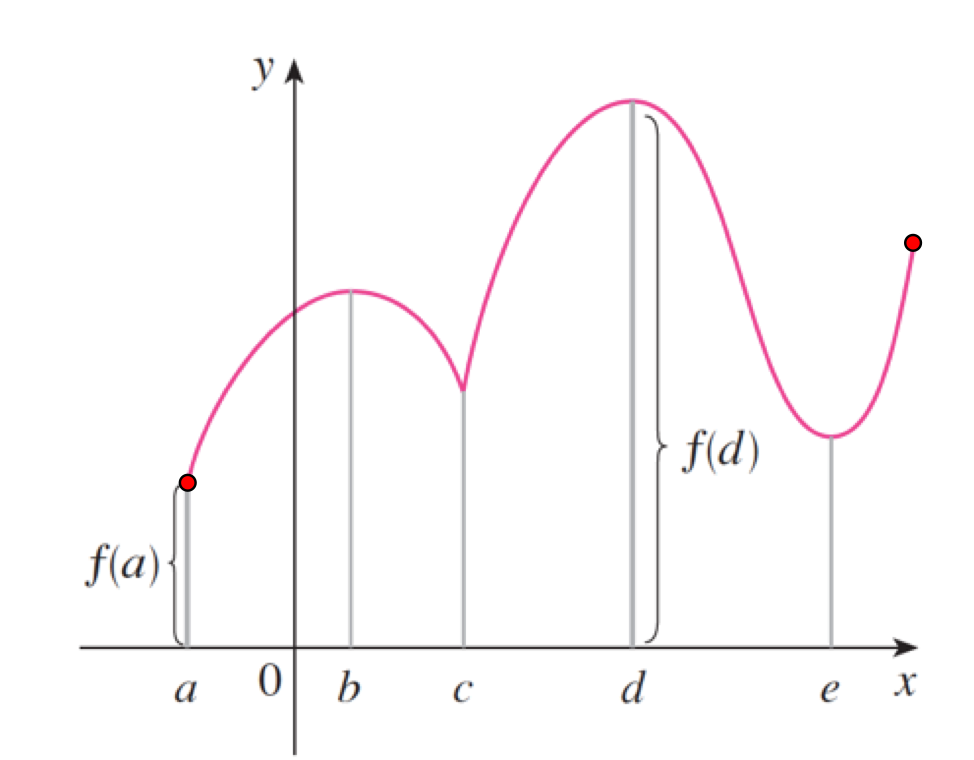
\includegraphics[width=7cm]{Graph_1.png}
\end{figure}
\subsection*{Example 3} The graph of the function $f(x)=3x^4-16x^3+18x^2$ on the domain $-1\leq x\leq 4$ is below. State the local maximum and minimum values of the function. For abs. max/min state whether it is an endpoint or interior point.
\begin{figure}[h]
    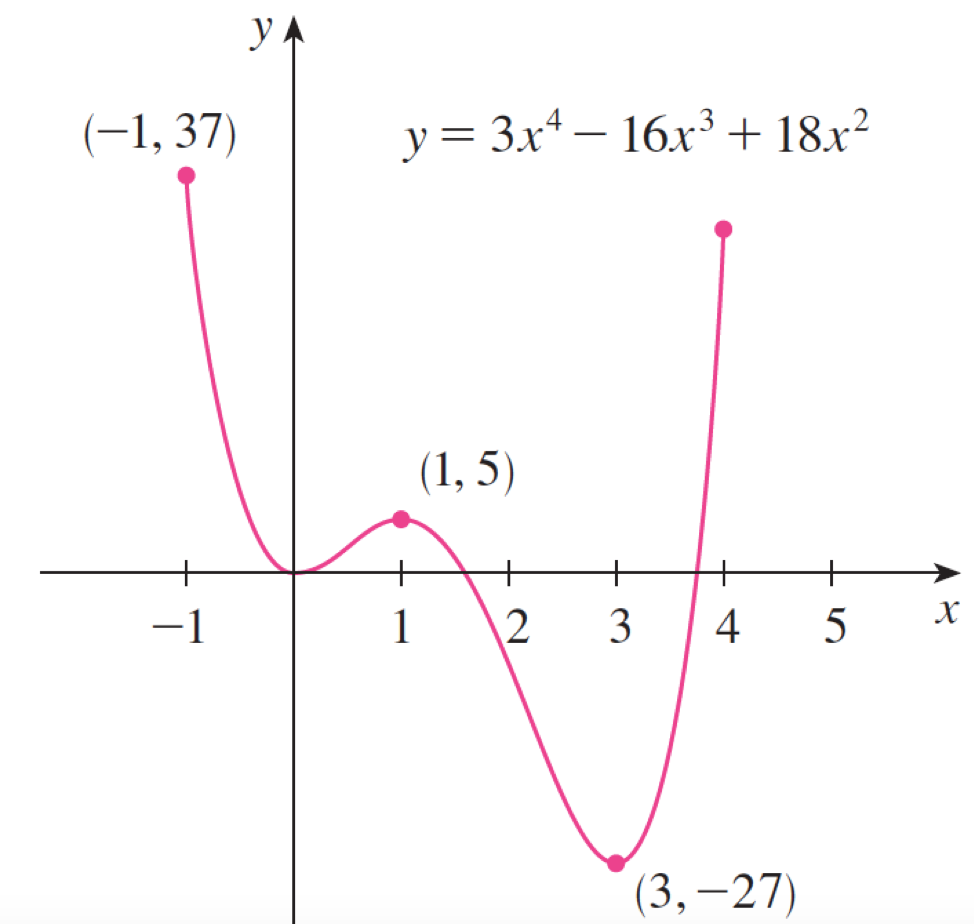
\includegraphics[width=6.5cm]{Graph_4.png}
\end{figure}
\clearpage
\begin{tcolorbox}
\subsection*{Theorem: Extreme Values}
If $f$ is \underline{\hspace{3cm}} on a closed interval $[a,b]$, then $f$ has absolute maximum and absolute minimum values at $x$ values in $[a,b]$.\\ \\
In other words, for a (1) continuous function (2) on a closed interval we are guaranteed absolute maximum and minimum values.
\end{tcolorbox}
\begin{figure}[h]
    \centering
    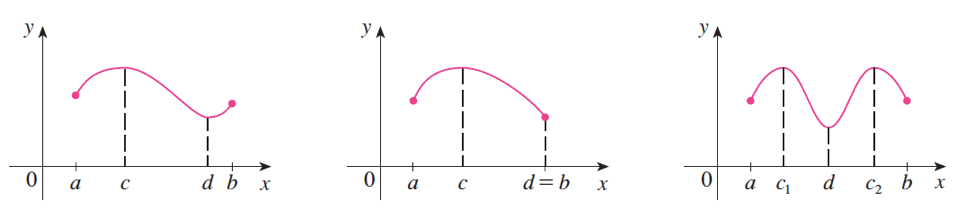
\includegraphics{Graph_5.png}
\end{figure}
\subsection*{Example 4} Below are the graphs of two functions. Explain why the Extreme Value Theorem cannot be applied. Indicate if there are any abs. max/min, explain your response.
\begin{figure}[h]
    \centering
    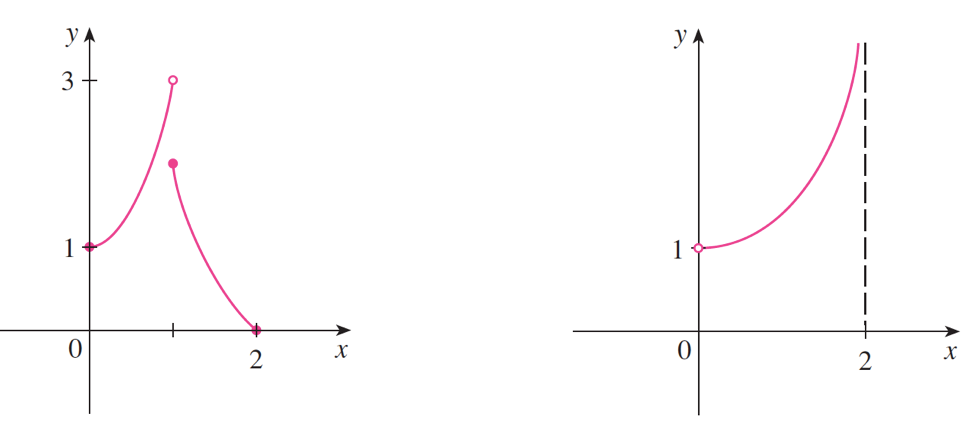
\includegraphics{Graph_6.png}
\end{figure}
\clearpage
\begin{tcolorbox}
\subsection*{Critical Numbers and Closed Interval Method}
\textbf{Definition:} A CRITICAL NUMBER of a function $f$ is a number $c$ in the domain of $f$ such that $f'(c)=0$ OR $f'(c)$ does not exist.\\ \\
\textit{Remark:} If a function has local max/min at $c$, then $c$ \underline{is} a critical number. The converse is not necessarily true, if $f'(c)=0$, this does not imply you have local max/min.\\ \\
\textbf{Closed Interval Method to find abs. max/min of a \underline{continuous} function on a \underline{closed interval} $[a,b]$}
\begin{enumerate}
    \item Find the critical numbers in $(a,b)$,
    \item Evaluate $f$ at the critical numbers and at endpoints,
    \item Pick the largest/smallest values from step (2).
\end{enumerate}
\end{tcolorbox}
\subsection*{Example 5} Find the critical numbers of $f(x)=x^{3/5}(4-x)$\vspace{5cm}
\subsection*{Example 6} Find the absolute maximum and minimum values of the function 
\[
f(x)=x^3-3x^2+1\textrm{ on $-\frac{1}{2}\leq x\leq 4$.}
\]
\end{document}